\section{Desarrollo del modelo Canvas}

\subsection{Segmentos de mercado}

El segmento prioritario corresponde a dueños y administradores de gimnasios
pequeños y medianos que necesitan conocer el estado de clientes, cobros,
membresías y asistencia. El segundo segmento comprende entrenadores personales
que gestionan varias personas y requieren organizar planes y progreso. Los
miembros son usuarios beneficiarios cuya adopción influye en la permanencia del
gimnasio como cliente.

La zona inicial es Pérez Zeledón. Se evita afirmar un tamaño de mercado hasta
contar con un directorio verificable y resultados de encuesta. El perfil de
cliente temprano propuesto es un establecimiento con administración concentrada
en una o pocas personas, acceso estable a internet y disposición para ejecutar
un piloto acompañado.

\begin{table}[H]
\caption{Segmentos y necesidades iniciales}
\begin{tabularx}{\textwidth}{>{\bfseries}p{3.3cm}X X}
\toprule
Segmento & Necesidad principal & Papel en el modelo \\
\midrule
Dueño o administrador & Controlar operación, cartera, vigencias y asistencia. & Comprador y responsable de adopción. \\
Entrenador & Organizar planes, sesiones y seguimiento. & Usuario profesional y posible comprador individual. \\
Miembro adulto & Consultar su plan, estado, asistencia y progreso. & Usuario beneficiario. \\
Personal autorizado & Ejecutar tareas administrativas delimitadas. & Usuario operativo futuro. \\
\bottomrule
\end{tabularx}
\caption*{\fuentepropia}
\end{table}

\subsection{Propuesta de valor}

GymHub centraliza información administrativa y deportiva con vistas adaptadas al
rol. Para el administrador, la propuesta es convertir datos dispersos en acciones
como revisar mora, activar membresías o detectar inactividad. Para el entrenador,
consiste en relacionar prescripción, ejecución y progreso. Para el miembro,
consiste en disponer de una ruta clara para consultar y registrar su actividad.

Los diferenciadores propuestos son enfoque local, acompañamiento inicial,
interfaz responsive y combinación de gestión con seguimiento. Ningún diferenciador
se presentará como ventaja comprobada hasta compararlo con alternativas comerciales
y obtener retroalimentación de personas usuarias.

\subsection{Canales}

Los canales se organizan según la etapa del vínculo:

\begin{itemize}
  \item \textbf{Conocimiento}: demostraciones breves, redes sociales, página
  informativa y recomendaciones.
  \item \textbf{Evaluación y venta}: visita o videollamada, diagnóstico básico,
  demostración y prueba piloto.
  \item \textbf{Entrega}: plataforma web responsive y configuración inicial.
  \item \textbf{Soporte}: WhatsApp Business, correo y material de ayuda.
\end{itemize}

La venta directa se prioriza en la fase institucional porque permite aprender del
cliente con un costo comercial bajo. La publicidad pagada se posterga hasta
comprobar qué problema y mensaje generan interés.

\subsection{Relaciones con clientes}

La relación propuesta combina incorporación asistida, soporte y revisión
periódica. El piloto debe comenzar con alcance, responsables y duración definidos.
Al cierre se evaluarán frecuencia de uso, incidencias, funciones utilizadas y
disposición de continuidad.

El servicio no debe depender permanentemente de soporte manual. Los tutoriales,
mensajes de error comprensibles y configuración guiada deben reducir consultas,
mientras el contacto humano se reserva para adopción, problemas de cuenta y
retroalimentación relevante.

\subsection{Fuentes de ingresos}

La fuente principal es la suscripción mensual por gimnasio. Como extensiones
futuras se consideran configuración especializada, soporte prioritario y módulos
adicionales. Los precios de la Tabla~\ref{tab:planes} son hipótesis para consultar
en la encuesta, no tarifas validadas.

\begin{table}[H]
\caption{Planes comerciales provisionales}
\label{tab:planes}
\begin{tabularx}{\textwidth}{>{\bfseries}p{2.5cm}X r p{2.2cm}}
\toprule
Plan & Alcance propuesto & Precio mensual & Estado \\
\midrule
Entrenador & Clientes individuales, planes y progreso. & CRC 7\,500 & Hipótesis \\
Básico & Miembros, membresías, pagos y asistencia. & CRC 15\,000 & Hipótesis \\
Intermedio & Básico, planes, sesiones, progreso y reportes. & CRC 25\,000 & Hipótesis \\
Avanzado & Intermedio, alertas y automatizaciones disponibles. & CRC 40\,000 & Hipótesis futura \\
\bottomrule
\end{tabularx}
\caption*{\textit{Nota}. Elaboración propia. Los montos deben ajustarse con los resultados de disposición de pago, 2026.}
\end{table}

\subsection{Recursos clave}

\begin{longtable}{>{\bfseries}p{3.3cm}p{11.2cm}}
\caption{Recursos clave de GymHub}\label{tab:recursos}\\
\toprule
Categoría & Recursos \\
\midrule
\endfirsthead
\toprule
Categoría & Recursos \\
\midrule
\endhead
Físicos & Computadoras disponibles, teléfonos de prueba, conexión a internet y equipo de demostración. \\
Tecnológicos & Código fuente, frontend, API, base PostgreSQL, despliegue web, repositorio, herramientas de prueba y sistema de respaldo. \\
Intelectuales & Conocimiento de programación, diseño de interfaces, bases de datos, seguridad, documentación y modelo de negocio. \\
Humanos & Dos estudiantes con responsabilidades compartidas, docente tutor, personas piloto y posibles responsables de gimnasios aliados. \\
Financieros & Suscripción de desarrollo, infraestructura de nube comercial futura, dominio y reserva para contingencias. \\
\bottomrule
\caption*{\fuentepropia}
\end{longtable}

\subsection{Actividades clave}

Las actividades centrales son investigación, priorización del producto,
desarrollo, pruebas, despliegue, documentación, demostración, incorporación de
clientes y soporte. El equipo comparte responsabilidades para evitar atribuciones
que no han sido documentadas individualmente.

\begin{table}[H]
\caption{Actividades, responsables y evidencia}
\begin{tabularx}{\textwidth}{>{\bfseries}p{3.5cm}p{2.7cm}X X}
\toprule
Actividad & Responsable & Recurso & Evidencia \\
\midrule
Investigación de mercado & Equipo & Encuesta y entrevistas & Resultados pendientes. \\
Desarrollo y corrección & Equipo & Repositorio y ambiente local & Historial y pruebas. \\
Diseño de datos y API & Equipo & Django, DRF y PostgreSQL & Modelos, endpoints y esquema. \\
Interfaz y experiencia & Equipo & React y herramientas frontend & Pantallas y pruebas. \\
Validación técnica & Equipo & Suite automatizada y demo & Reportes y compilaciones. \\
Revisión académica & Equipo y tutor & Lineamientos ExpoTÉCNICA & Lista de cumplimiento. \\
Piloto y soporte & Equipo & Gimnasio aliado & \pendiente{} \\
\bottomrule
\end{tabularx}
\caption*{\fuentepropia}
\end{table}

\subsection{Alianzas clave}

Las alianzas iniciales aportan conocimiento y validación antes que capital. Se
requiere un gimnasio piloto, responsables que respondan la encuesta, miembros
adultos, el docente tutor y apoyo técnico puntual. Si se amplía el módulo de
alimentación, se deberá incorporar una persona profesional competente antes de
ofrecer orientación personalizada.

\begin{table}[H]
\caption{Alianzas requeridas}
\begin{tabularx}{\textwidth}{>{\bfseries}p{3.4cm}X X p{2.3cm}}
\toprule
Aliado & Aporte & Beneficio & Estado \\
\midrule
Gimnasio local & Contexto, prueba y retroalimentación. & Validación operacional. & Pendiente \\
Entrenador & Revisión de flujo de planes y sesiones. & Pertinencia deportiva. & Pendiente \\
Miembros adultos & Pruebas de comprensión y utilidad. & Mejora de experiencia. & Pendiente \\
Docente tutor & Revisión académica y administrativa. & Cumplimiento. & Activo \\
Proveedores de nube & Infraestructura tecnológica. & Despliegue y escalamiento. & En uso \\
\bottomrule
\end{tabularx}
\caption*{\fuentepropia}
\end{table}

\subsection{Estructura de costos}

Los costos se separan en desembolsos actuales, aportes en especie e infraestructura
comercial. Esta clasificación evita afirmar que el desarrollo es gratuito cuando
utiliza equipo, internet y tiempo. El detalle y los escenarios se presentan en la
sección de costos e ingresos.

\subsection{Representación visual}

La Figura~\ref{fig:canvas} resume el Canvas inicial recuperado del documento de
referencia. Sus montos y afirmaciones deben interpretarse junto con las
aclaraciones de este escrito.

\begin{figure}[H]
\centering
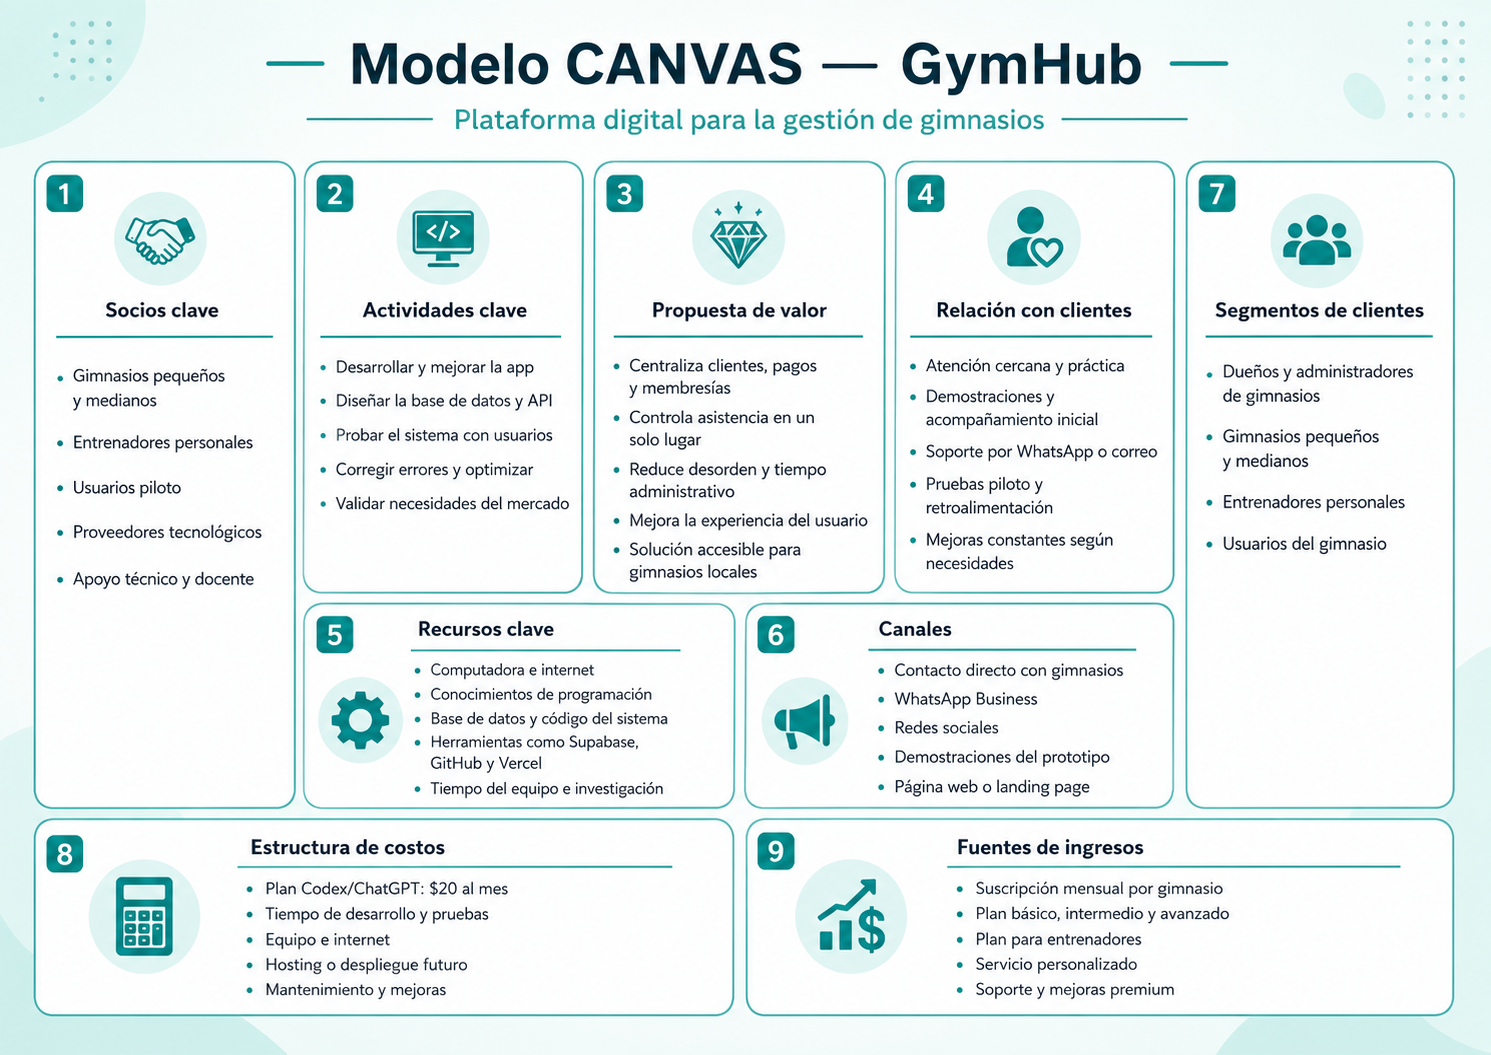
\includegraphics[width=\textwidth]{imagenes/canvas_gymhub.png}
\caption{Modelo Canvas inicial de GymHub}
\label{fig:canvas}
\caption*{\textit{Nota}. Elaboración propia a partir del documento inicial del equipo, 2026.}
\end{figure}
